% Copyright (c) 2003-2021 Robert Ryszard Paciorek <rrp@opcode.eu.org>
% 
% MIT License
% 
% Permission is hereby granted, free of charge, to any person obtaining a copy
% of this software and associated documentation files (the "Software"), to deal
% in the Software without restriction, including without limitation the rights
% to use, copy, modify, merge, publish, distribute, sublicense, and/or sell
% copies of the Software, and to permit persons to whom the Software is
% furnished to do so, subject to the following conditions:
% 
% The above copyright notice and this permission notice shall be included in all
% copies or substantial portions of the Software.
% 
% THE SOFTWARE IS PROVIDED "AS IS", WITHOUT WARRANTY OF ANY KIND, EXPRESS OR
% IMPLIED, INCLUDING BUT NOT LIMITED TO THE WARRANTIES OF MERCHANTABILITY,
% FITNESS FOR A PARTICULAR PURPOSE AND NONINFRINGEMENT. IN NO EVENT SHALL THE
% AUTHORS OR COPYRIGHT HOLDERS BE LIABLE FOR ANY CLAIM, DAMAGES OR OTHER
% LIABILITY, WHETHER IN AN ACTION OF CONTRACT, TORT OR OTHERWISE, ARISING FROM,
% OUT OF OR IN CONNECTION WITH THE SOFTWARE OR THE USE OR OTHER DEALINGS IN THE
% SOFTWARE.

\documentclass[fontSize=10pt, extra]{pdfArticle}

% include Examples related functions
\input{LaTeX-demos-examples.tex}

\usepackage{xfrac} % ułamki ukośne

\usepackage{pgfplots} % wykresy

\usepackage{tikz}
\usetikzlibrary{positioning} % for positionig nodes with `right = of X`
\usetikzlibrary{automata} % for initial and accepting nodes in tikzpicture graphs
\usetikzlibrary{arrows.meta, decorations.markings} % for arrows formating in tikzpicture
\usetikzlibrary{shapes} % for elipse nodes

\usepackage{tikz-timing}
\usetikztiminglibrary{either}

\usepackage{tikzPackets}

\newenvironment{ExampleVerticalBox}{
	\VerbatimEnvironment
	\begin{CatchExample}%
}{%
	\end{CatchExample}
	\putExampleVerbatimAdjust
	
	\begin{adjustwidth}{1cm}{7cm}%
		\putExampleTeX%
	\end{adjustwidth}%
}
\newenvironment{ExampleSmallCode}{
	\VerbatimEnvironment
	\begin{CatchExample}%
}{%
	\end{CatchExample}
	\nopagebreak
	
	\hspace{0.015\textwidth}\parbox[c]{0.4\textwidth}{%
		\vspace{-\topsep}\vspace{-\partopsep}\vspace{-\parskip}%
		\putExampleVerbatim%
		\vspace{-\topsep}\vspace{-\partopsep}%
	}%
	\hspace{0.03\textwidth}\parbox[c]{0.5\textwidth}{\centering%
		\putExampleTeX%
	}%
}

\begin{document}

\section{Różności}

\subsection{Komentarze}
Oprócz klasycznych komentarzy (od \Verb@%@ do końca linii) możemy też użyć komentarza blokowego:
\begin{Verbatim}
  \begin{comment}
    komentarz wieloliniowy
    ALA MA KOTA
  \end{comment}
\end{Verbatim}
Także tekst za \Verb@\end{document}@ jest ignorowany będąc swego rodzaju komentarzem.


\subsection{Matematyka}
Przedstawie tu tylko wybrane elementy związane z składem wyrażeń matematycznych - po pełwn opis (w tym listę różnych symboli) odsyłam do rozdziału trzeciego \href{ftp://ftp.gust.org.pl/TeX/info/lshort/polish/lshort2e.pdf}{Nie za krótkie wprowadzenia do systemu LaTeX 2e} oraz innych źródeł.

\vspace{0.3cm}
\noindent\begin{ExampleVerticalBox}
dwumiany bez nawiasów / z nawiasami:
	${a \atop b}$ / ${a \choose b}$
\\
ułamki:
	${a \over b}$ lub $\frac{a}{b}$
\\
ułamki ukośne (zdefiniowane w xfrac):
	$\sfrac{a}{b}$
\end{ExampleVerticalBox}

\noindent\begin{ExampleVerticalBox}
linia nad / pod jakimś wyrażeniem:
	$\overline{a+b}$ / $\underline{a+b}$
\\
napis nad strzałką:
	$\stackrel{a}{\rightarrow}$
\\
klamra pod / nad wyrażeniem (z podpisem pod / nad klamrą):
	$\underbrace{2+3}_{5}$ / $\overbrace{2+3}^{5}$
\end{ExampleVerticalBox}

\noindent\begin{ExampleVerticalBox}
\newcommand\minifrac[2]{%
	\raisebox{.3ex}{$#1$}/\raisebox{-.6ex}{$#2$}
}
\newcommand\inpoint[1]{%
	\hspace{.4ex}\raisebox{-.55ex}{\scalebox{0.7}{$\bigg|_{#1}$}}\hspace{-.8ex}
}
%
ułamek a/b z różnicą wysokości zapisu a i b:
	$\minifrac{5}{13}$
\\
kreska "w punkcie" np. do pochodnej:
	$A \inpoint{2x}$
\end{ExampleVerticalBox}

% Interesujący jest też pakiet \href{http://mirrors.ctan.org/macros/latex/contrib/siunitx/siunitx.pdf}{siunitx} pozwalający na formatowanie liczb i jednostek
% \begin{Example}
% \sisetup{group-minimum-digits=4,negative-color=red}
% \num[group-separator={\,}]{1245.34}\\
% \num[output-decimal-marker={~}]{1245.34}\\
% \num{-12.8} \num[negative-color=]{-12.8}\\
% \SI[mode=text]{1.23}{J.mol^{-1}.K^{-1}}
% \end{Example}


\subsection{Bibliografia i bibtex}
Odnośniki do bibliografii wstawiamy poprzez \Verb#\cite{ID_pozycji_bibliograficznej}#. Samą bibliografię możemy utworzyć:
\begin{Verbatim}
 \begin{thebibliography}{99}
  \addcontentsline{toc}{chapter}{Bibliografia}
  \bibitem[identyfikatorWidoczny]{ID_pozycji_bibliograficznej}%
          Autor, \textit{Tytuł}, Miejsce publikacji i rok.
 \end{thebibliography}
\end{Verbatim}
Przy większych pracach warto skorzystać z systemu do tworzenia bibliografii bibtex, odwołania do pozycji tworzy się w identyczny sposób, a sam spis umieszcza się poprzez:
\begin{Verbatim}
 \cleardoublepage\phantomsection%
   \addcontentsline{toc}{chapter}{Bibliografia}
 \bibliographystyle{plunsrt}\nocite{*}%
   \bibliography{nazwa_pliku_z_bibliografia}
\end{Verbatim}
Budowanie latex'a z zastosowaniem bibtexa wymaga wydania dodatkowo komendy bibtex nazwa\_bez\_rozszerzenia przed budowaniem właściwego pliku latex'a. Sam plik bibliograficzny składa się z rekordów postaci (więcej na ten temat w Bibliografia w LaTeXu - program bibtex):
\begin{Verbatim}
@misc{ID_pozycji_bibliograficznej,
	author        = "",
	title         = "",
	journal       = "",
	year          = "",
	volume        = "",
	school        = "",
	url           = "",
	institution   = "",
	howpublished  = "",
	type          = ""
}
\end{Verbatim}


\subsection{Liczniki}

Liczniki przydają się do automatycznej numeracji rozdziałów, paragrafów itp. Liczniki tworzymy poleceniem \Verb#\newcounter{nazwa_licznika}#, wartość nadajemy mu poprzez \Verb#\setcounter{nazwa_licznika}{wartosc}#, zwiększać możemy ją o jeden poprzez instrukcję \Verb#\stepcounter{nazwa_licznika}#.
Wartość licznika może być wstawiona (wyświetlona) na kilka sposobów (zależnie od pożądanego formatu). Na przykład:
\begin{itemize}
	\item \Verb#\Roman{nazwa_licznika}# – wielkie liczby rzymskie,
	\item \Verb#\Alph{nazwa_licznika}# – wielkie litery,
	\item \Verb#\alphalph{nazwa_licznika}# – małe litery  - wersja obsługująca numerację powyżej \textit{z} jako \textit{aa}, \textit{ab}, itd.,
	\item \Verb#\arabic{nazwa_licznika}# – liczby arabskie
\end{itemize}

Poniższy przykład ilustruje sposób umieszczania automatycznych odwołań do zadanych fragmentów pliku (np. paragrafów jakiegoś regulaminu).

\begin{Verbatim}
% wlaczam plik z definicjami liczników
\IfFileExists{\jobname.cou}{\input{\jobname.cou}}{}

% otwieram do zapisu plik z baza odnośników i zapisuje nagłówek
\newwrite\licznfile
\openout\licznfile=\jobname.cou
\write\licznfile{\string\def\string\liczniki{}}

% ustawiamy zamknięcie plik z licznikami w /end{document}
\AtEndDocument{\closeout\licznfile} 

% instrukcja zapamiętuje licznik w pliku (jako licznik o zadanej nazwie)
% \zapamietajlicznik{nazwa_licznika_do_zapamietania}{nazwa_nowego_licznika}
% przy czym dla środowiska enumerate są to dla kolejnych poziomów:
%  enumi enumii enumiii enumiv ...
\newcommand{\zapamietajlicznik}[2] {
  \immediate\write\licznfile{
    \string\newcounter{#2}\string\setcounter{#2}{\arabic{#1}}
  } % \string - zabezpiecza backslesh (\)
}

% nie tworze liczników przy pierwszym obiegu - zamiast nich będę wpisywał XXX
% dopiero po wczytaniu ich z pliku wstawię odpowiednie numerki
\newcommand{\alphf}[1]{\ifx \liczniki \undefined XXX \else\alph{#1}\fi}
\newcommand{\arabicf}[1]{\ifx \liczniki \undefined XXX \else\arabic{#1}\fi}

% W miejscu do którego chcemy się odwołać
% umieszczamy instrukcję zapamiętania licznika:
%  \zapamietajlicznik
%     {nazwa_zapamietywanego_licznika}
%     {nazwa_pod_ktora_chemy_go_zapamietac}.
%
% W miejscu w którym chcemy wstawić odwołanie umieszczamy np:
%  \arabicf{nazwa_pod_ktora_zapamietalismy_licznik}
\end{Verbatim}


\subsection{Wczytywanie plików i informacje o pliku}

Poniższy przykład:
\begin{enumerate}
	\item wykonuje polecenie shellowe generujące plik z sumą kontrolną i pełną ścieżką do źródła
	\item używa pakietu \textit{} do wczytania tego pliku
	\item pozwala na wstawienie tych informacji w treści dokumentu (np. w stopkach)
\end{enumerate}

\noindent\begin{ExampleVerticalBox}
\newcommand\CatchRawTextFile[2]{
  \CatchFileEdef{#1}{#2}{
    \catcode`\#=12 \catcode`\$=12 \catcode`\%=12 \catcode`\&=12 \catcode`\\=12
    \catcode`\^=12 \catcode`\_=12 \catcode`\{=12 \catcode`\}=12 \catcode`\~=12
  }
}

\def\FileMDSum{}
\def\FileName {\jobname.tex}
\def\FilePath {}

\newcommand{\getMDSum}{
  % obliczenie md5 pliku źródłowego i wczytanie do rejestru \SrcFileInfo
  \immediate\write18{echo "`md5sum \jobname.tex` `pwd`/" > \jobname.info.md5}
  \IfFileExists{\jobname.info.md5}
    {\CatchRawTextFile{\SrcFileInfo}{\jobname.info.md5}}
    {\ClassError{office}
      {Can't find/generate md5 file (use h for help)}
      {You can:
        \MessageBreak\space - run pdflatex with --shell-escape to generate md5 sum
        \MessageBreak\space - run before pdflatex:
        \MessageBreak\space\space\space\space  echo '`md5sum "\jobname.tex"` `pwd`/' > "\jobname.info.md5"
      }
    }
  \immediate\write18{rm \jobname.info.md5}
  
  % podział wczytanej informacji na pola
  \let\FileMDSum\relax \let\FileName\relax \let\FilePath\relax
  \def\FileMDSum{\StrBefore[1]{\SrcFileInfo}{ }}
  \def\FileName {\StrBetween[1,2]{\SrcFileInfo}{ }{ }}
  \def\FilePath {\StrBehind[2]{\SrcFileInfo}{ }}
}

\getMDSum

Suma kontrola md5 dla pliku źródłowego \textit{\FileName{}} to:\\ \FileMDSum
\end{ExampleVerticalBox}

\subsection{Postscript}
LaTeX umożliwia także zaawansowane zabawy z włączanymi plikami postscriptowymi. Przy użyciu pakietu "psfrag" możemy dokonywać podmiany napisów w EPS:
\begin{Verbatim}
  \psfrag{tekst_do_zastapienia}{
  tekst zastępujący \small{może} zawierać np. $wzory$
  }
  \psfragscanon
  \nopagebreak\newline\centerline{
    \includegraphics[scale=0.7]{plot.eps}
  }
  \psfragscanoff
\end{Verbatim}

Możliwe jest także mieszanie PS i Latex (umieszczanie komend PS wewnątrz pliku latexowego):
\begin{Verbatim}
  \psset{linewidth=1mm}
  \begin{pspicture}(3,2)
    \pscurve[arrows=<->](0,1.3)(0.7,1.8)
    (3.5,0.7)(4,1.9)(0.4,0.4)
  \end{pspicture}
\end{Verbatim}


\subsection{Zaawansowana grafika z użyciem Ti\textit{k}Z / PGF}

Jest to system do tworzenia zaawansowanych rysunków z użyciem \LaTeX'a. Oprócz głównej biblioteki - \href{http://www.ctan.org/pkg/pgf}{Ti\textit{k}Z / PGF} istnieje wiele specjalistycznych \href{http://www.ctan.org/tex-archive/graphics/pgf/contrib}{pakietów z niej korzystających} - np:
\begin{itemize}
\item \href{http://www.ctan.org/pkg/pgfplots}{pgfplots} – umożliwia generowanie wykresów 2D (w tym histogramów) i 3D
\item \href{http://www.ctan.org/pkg/pgf-pie}{pgf-pie} – umożliwia generowanie wykresów kołowych
\item \href{http://www.ctan.org/pkg/tikzpackets}{tikzPackets} – umożliwia generowanie ilustracji nagłówków / ramek protokołów
\end{itemize}


\subsubsection{Ilustracje}

\noindent\begin{Example}
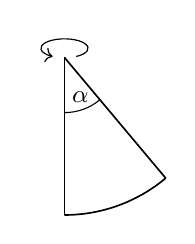
\begin{tikzpicture}[semithick]
  \node[yshift=1mm] {
    \tikz [x=0.12cm,y=0.30cm,line width=.1ex,->,rotate=90]
          \draw (0,0) arc (-150:150:1 and 1);
  };
  \draw[thin] (0,0) -- ++(270:2cm);
  \draw (0,0) -- ++(310:2cm);
  \draw ([shift=(270:2cm)]0,0) arc (270:310:2cm);
  
  \node[yshift=-5mm,xshift=2mm] {\small$\alpha$};
  \draw[thin] ([shift=(270:7mm)]0,0) arc (270:310:7mm);
\end{tikzpicture}
\end{Example}

\noindent\begin{Example}
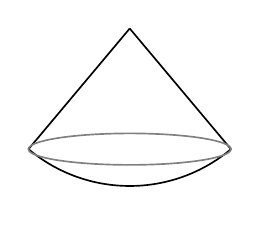
\begin{tikzpicture}[semithick]
  \draw (0,0) -- ++(230:2cm);
  \draw (0,0) -- ++(310:2cm);
  \draw ([shift=(230:2cm)]0,0) arc (230:310:2cm);
  \draw[gray] ([yshift=-2cm * cos{40}]0,0)
              ellipse (2cm * sin{40} and 0.2cm);
\end{tikzpicture}
\end{Example}

\subsubsection{Grafy}

\begin{ExampleVertical}
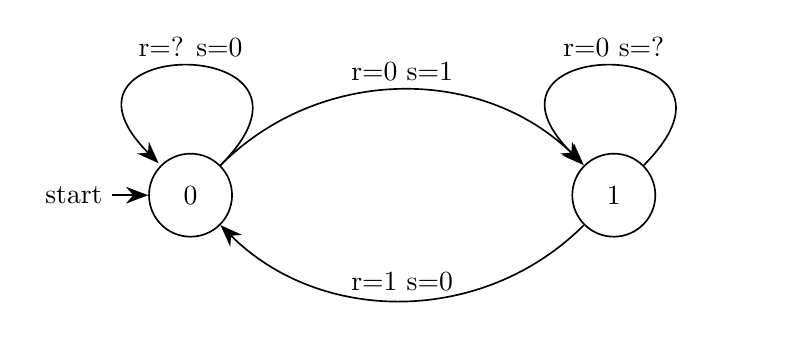
\begin{tikzpicture}[->, >={Stealth[length=8pt,width=6pt]}, node distance=4.3cm, semithick]
\node[circle, minimum size=3em, draw, initial] (0) {0};
\node[circle, minimum size=3em, draw] (1) [right = of 0] {1};
\path (0)  edge [bend left=45] node[above] {r=0 s=1} (1);
\path (1)  edge [bend left=45] node[above] {r=1 s=0} (0);

\path (0)  edge [loop] node[above] {r=? s=0} (0);
\path (1)  edge [loop] node[above] {r=0 s=?} (1);
\end{tikzpicture}
\end{ExampleVertical}

\subsubsection{Przebiegi czasowe}

Pakiet \textit{tikz-timing}:

\noindent\begin{Example}
\begin{tikztimingtable}[timing/U/background/.style={fill=red},]
 Name & hLLLLh \\
 Clock & 10{c} \\
 Signal & z[[timing/slope=.8]]4D{Text}zzH \\
 Test & H[[timing/slope=.5]]ZD[[timing/slope=.7]]DZ \\
 Test2 & LUUH\\
\end{tikztimingtable}
\end{Example}

\subsubsection{Nagłówki protokołów}

Pakiet \textit{tikzPackets}:

\noindent\begin{ExampleVertical}
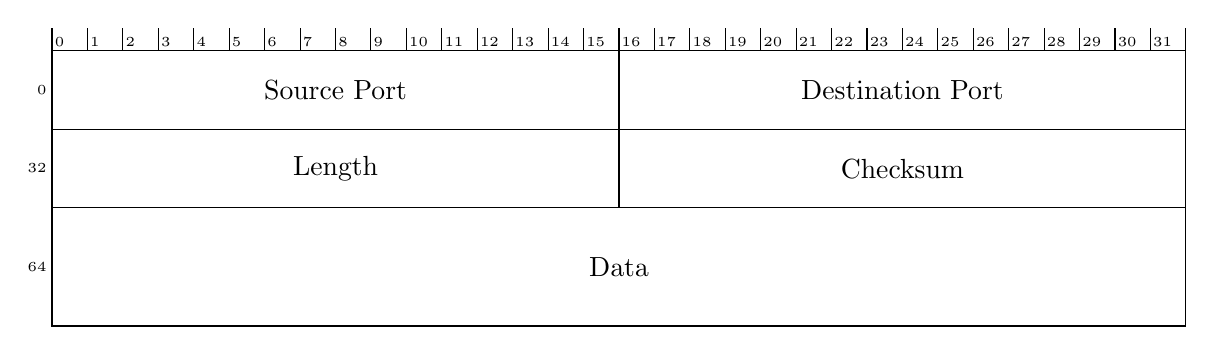
\begin{tikzpicture}
    \packetsInit
    \packetsBitWidth=4.5mm
    \packetsPrintBitScale{31}
    
    \packetsPutField{16}{Source Port}
    \packetsPutField{16}{Destination Port}
    \packetsEndLine{0}{}
    
    \packetsPutField{16}{Length}
    \packetsPutField{16}{Checksum}
    \packetsEndLine{32}{}
    
    \packetsPutField[protocolsField, minimum height=1.5cm]{32}{Data}
    \packetsEndLine{64}{}
\end{tikzpicture}
\end{ExampleVertical}


\subsubsection{Wykresy}

Pakiet \textit{pgfplots}:

\begin{ExampleSmallCode}
\begin{tikzpicture}
\begin{axis}
	\addplot coordinates {
		(1,1) (11,3) (13,3) (17,9)
	};
\end{axis}
\end{tikzpicture}
\end{ExampleSmallCode}


\copyrightFooter{
	© Robert Ryszard Paciorek <rrp@opcode.eu.org>, 2003-2021.\\
	Kopiowanie, modyfikowanie i redystrybucja dozwolone pod warunkiem zachowania informacji o autorach.
}
\end{document}
